\chapter{State of art}\label{03StateOfArt}
\noindent
Cooperative and non cooperative Sense and Avoid (SAA) systems are key enablers for Unmanned Aircraft (UAV) to routinely access non-segregated airspace \cite{spriesterbach2013unmanned}. Both cooperative and non-cooperative SAA systems are being developed to address this integration requirement.
\noindent
The SAA capability is defined as the automatic detection of possible conflicts by the UAV platform under consideration and performing avoidance maneuver tasks to prevent the identified collisions. An analysis of the available SAA candidate technologies and the associated sensors for both cooperative and non-cooperative SAA systems is presented in \cite{muraru2011critical}. Non-cooperative Collision Detection and Resolution (CD\&R) for UAV is considered as one of the major challenges that needs to be addressed \cite{lai2012see} for the insertion of UAVs in non-segregated air space. As a result, a number of non-cooperative sensors for the SAA system have been adopted. Light Detection and Ranging (LIDAR)is used for detecting, warning and avoiding obstacles for low-level flying \cite{sabatini2014lidar}.

An approach to the definition of encounter models and their applications to SAA strategies is presented in \cite{kochenderfer2008encounter} for both cooperative and non-cooperative scenarios.

Since 2014, there is a visible strong political support for developing rules on drones but regulations are not harmonized yet. The European Aviation Safety Agency (EASA) has been tasked to develop a regulatory framework for drone operations and proposals for the regulation of "low-risk" UAV operations. In achieving this, EASA is working closely with the Joint Authorities for Regulation of Unmanned Systes (JARUS) \cite{jarus2016regulations}.


\section{UAV motion model}
\noindent
This section strongly follows \cite{lee2011structure}.

\subsection{Continuous-time systems}\noindent
%This is very imprecise. A good notation is:
%1. u is the control function. It is a map from a time interval to \R^p, i.e., u:[0,T] \to %\R^p. Thus you could write u\in \C^p
%2. u(t) is the value (in \R^p) of the control function u. It is correct to write u(t)\in %\R^p

%You have to say what \C^p is. I guess that you mean the space of continuous functions. If this is the case, this specification is very unnatural since this space is too restrictive. Controls of interest usually have discontinuities.  More common is L^1 (space of integrable functions).

\noindent Consider a class of systems given by functions:
\begin{equation}
    \begin{split}
    S&: \vec{u}(t)  \to \vec{x}(\vec{x}_0,t) \\
    \vec{u}&(t): [0,T] \to \R^p \\
    \vec{u}&(t)\in \mathbb{R}^p , \vec{x}(t) \in \mathbb{R}^n \\
    \end{split}
\end{equation}
where $\vec{u}(t)$ and  $\vec{x}(\vec{x}_0,t)$ are a sets of continuous-time signals.
These are often called continuous-time systems because they operate on
continuous-time signals. Frequently, such systems can be defined by differential
equations that relate the input signal to the output signal.
A prototypical description of a controlled (there is a control input signal)
continuous-time system is:
\begin{equation}\label{eq:nonlinearsystem}
    \dot{x}(t) = f(t,x(t),u(t)), u(t) \in U(t)
\end{equation}
where $f:\mathbb{R}\times\mathbb{R}^n\times\mathbb{R}^p\to\mathbb{R}^n$
satisfies the conditions for existence
and uniqueness of the ordinary differential equation and $u$ is our control\cite{butcher1987numerical}.

\subsection{Discrete-time systems}
\noindent
\noindent Consider another class of systems given by functions
\begin{equation}\label{eq:Discretegenericuavmodel}
    \begin{split}
    S&: \vec{u}(k)  \to \vec{x}(k), \\
    k& \in \{0, t_s, 2.t_s, 3.t_s, \dots i.t_s\}, i \in \N^+\\
    \vec{u}&(k)\in \mathbb{R}^p , \vec{x}(k) \in \mathbb{R}^n\\
    \end{split}
\end{equation}
where $\vec{u}(k), \vec{x}(k)$ is a set of discrete-time signals. They can be represented by a function $f$ like $f:\{0, t_s, 2.t_s, 3.t_s, \dots i.t_s\} \to \R^n,  i \in \N^+$ where $t_s$ is sampling time and $i$ is discrete step \cite{shampine1997matlab}.

% REACH SETS
\section{Reach sets}\label{s:ReachSets}
\noindent
The reach set of a system described by a differential equation is the
set of all states that can be reached from an initial state within a given time
interval.
\noindent For general case consider the system described by equation (\ref{eq:nonlinearsystem}).

\begin{definition}[Reach set starting at a given point]\label{def:reachset01}
Suppose the initial position
and time $(\vec{x}_0, t_0)$ are given. The reach set $\mathscr{R}[\tau; t_0, \vec{x}_0]$ of system (\ref{eq:nonlinearsystem}) at time $\tau \ge t_0$, starting at position and time $(\vec{x}_0, t_0)$ is given by:
\begin{equation}\label{eq:basicReachSetDefinition}
    \mathscr{R}[\tau, t_0, \vec{x}_0] = \bigcup \{\vec{x}(\tau):\vec{u}(s)\in U(s),s \in (t_0,\tau]\}
\end{equation}
\end{definition}
\noindent Reach set starting at given set can be used to determine reach set in case of hybrid system input control switch and it is defined as follow:
\begin{definition}[Reach set starting at a given set]
The reach set at time $\tau > t_0$ starting from set $X_0$ is defined as:
\begin{equation}
    \mathscr{R}[\tau, t_0, X_0] = \bigcup \{R[\tau, t_0, \vec{x}_0]:\vec{x}_0 \in X_0\}
\end{equation}
\end{definition}

\noindent Reach set for adversarial behavior can be used to calculate possible escape routes from pursuer and it is defined as follow:
\begin{definition}[Reach set under adversarial behavior]
Consider now the case of adversarial behavior, for system $\dot{x}=u,u\in \mathbb{B}$.
where $u(t)$ is our control and $v(t)$ is adversary control which is independent of $u(t)$, let $w(t)=u(t)- \arg_{v(t)\in V(t)}\sup_{{x} \in x(t)} v(t)$, which represents worst possible input change in given state and time, then reach set for system is represented as:
\begin{equation}
    \mathscr{R}[\tau; t_0, \vec{x}_0] = \bigcup \{\vec{x}(\tau):\vec{w}(s) \in W(s),s \in (t_0,\tau]\}
\end{equation}

\end{definition}

\noindent Reach set under constraints are usable to define state constrained systems in terms of dynamics and technical capabilities.
\begin{definition}[Reach set under state constraints]
Suppose the initial position
and time $(\vec{x}_0, t_0)$ and $x$ constraints are given $x(t) \in \mathbb{A} \subset \R^n, \dot{x}(t) \in \mathbb{B} \subset \R^n$. The reach set $\mathscr{R}[\tau, t_0, \vec{x}_0]$ of system (\ref{eq:nonlinearsystem}) at time $\tau \ge t_0$, starting at position and time $(\vec{x}_0, t_0)$ is given by:
\begin{equation}
    \mathscr{R}[\tau, t_0, \vec{x}_0] = \bigcup \{\vec{x}(\tau):\forall s\in (t_0,\tau], x(s) \in \mathbb{A}, \dot{x}(s) \in \mathbb{B}, \exists u(s) \in U(s)\}
\end{equation}
\end{definition}


\section{Occupied space}
\noindent Occupied space representation is crucial in obstacle avoidance, this section introduces models and notations. Analytical geometry structures of sphere and ellipsoid are used to  determine closed occupied spaces.
\begin{definition}{Unit sphere (Unit ball) $\mathscr{B}(\vec{p},r)$} denotes occupied space in point $\vec{p} = [x_p,y_p,z_p]^T$ with radius $r$. Where point $\vec{b} = [x_b,y_b,z_b]$ belongs to sphere $\mathscr{B}(\vec{p},r)$ if and only if:
\begin{equation}
    (x_b-x_p)^2 + (y_b-y_p)^2 + (z_b-z_p)^2 \le r
\end{equation}    
\end{definition}
Definition of sphere $\mathscr{B}(\vec{p},r)$ is usually used to denote safety margin of vehicle $s_m$, where $s_m$ represents maximum radius to vehicle matter point from vehicle mass center. 
\begin{definition}{Spherical coating $\mathscr{C}(\vec{f}(\cdot),r)$} denotes occupied space of object which surface can be approximated by function $f(\cdot)$, with points of surface $\vec{p}=[x_p,y_p,z_p]^T\in\R^3$ and object inner points $\vec{i}=[x_i,y_i,i_p]^T\in \R^3$. Then spherical coating $\mathscr{C}(\vec{f}(\cdot),r)$ is defined as follows:
\begin{equation}
    \mathscr{C}(\vec{f}(\cdot),r) = \left\{\vec{b} \in \R^3: \vec{b}\in \bigcup_{\forall \vec{p} \in \vec{f}(\cdot)} \mathscr{B}(\vec{p},r), \nexists \vec{i}=\vec{b}  \right\}
\end{equation}
One can say that spherical coating is a closed,not compact set of points $\vec{b} = [x_b,y_b,z_b]$  where distance to closest surface point $\vec{p}$ is lesser or equal to coating radius $r$.    
\end{definition}
\noindent Calculation of spherical coating can be time consuming especially when surface function $\vec{f}(\cdot)$ is not smooth \cite{sommerville2016analytical}. Closest point problem has been formulated by Shamos \cite{shamos1975closest}.Closest point estimation with moving vehicle and with thick data flow can by solved by time optimal and deterministic approach, one of them have been presented by Bentley in \cite{bentley1980optimal}. Approach is based on closest point search in local planar coordinates which may be ideal for steam-line LiDAR data. 
Estimation of spherical coating is used in potential field avoidance methods. One most notable study was using spherical approximation based on obstacle center and mass distribution in space \cite{borenstein1991vector}. Potential field have their limitations in partially known environment, because it is hard to determine center of mass and mass distribution of obstacle from partial information \cite{koren1991potential}. Main source of object proportional estimation can be reused from camera based solutions like \cite{oberkampf1993iterative}. Other possible solution sources from fast clustering algorithms from Geographical Information Systems (GIS) for example \cite{zaiane2002clustering}.

\section{Movement automaton}\label{sec:movement automaton}
\noindent Movement automaton used as proxy between discrete command chain (movement chain) and control signal ($u(t)$). Movement automation is based on hybrid automaton.
\begin{definition} {Hybrid automaton $\mathscr{H}(Q,\R^n,f,\varphi,\rho)$} is well defined system representation consisting from following components.
\begin{equation}
    \begin{aligned}
        Q &\equiv \textnormal{set of discrete states}\\
        \R^n &\equiv \textnormal{continuous state-space} \\
        f: Q\times \R^n \to \R^n & \equiv \textnormal{vector field}\\
        \varphi:Q\times \R^n \to Q & \equiv \textit{discrete transition}\\
        \rho : Q\times \R^n \to \R^n & \equiv\textit{reset map}\\
    \end{aligned}
\end{equation}
Discrete state $q_i \in Q$ represents system current state and impacts system behavioural equation and state. Continuous state $[x(t),u(t)]\in \R^n$ represents  system state from physical viewpoint (values of state variables and inputs in continuous space $\R^n$). Vector field $f$ assign to each discrete state $q_i \in Q$ system behavioral function $\dot{x} = f(x,u)$. Discrete transition $\varphi$ defines conditions to transit between two different states. Reset map $\rho$ defines system state or input change on reset conditions.
\end{definition} 

\begin{definition}{Trajectory primitive $\hat{t}(x_0,t_0,t_1)$} is defined on given time interval $(t_0,t_1]$ for system $\dot{x} = f(x,u)$ with initial state $x_0$ at $t_0$ and final state $x_1$ at $t_1$ as follow:
\begin{equation}
    \hat{t}(x_0,t_1,t_1) = \left\{ x\in\R^n: x = \Phi(t_0,\tau,x_0), \tau \in (t_0,t_1] \right\}
\end{equation}
Trajectory primitive can be viewed as ordered set of system trajectory positions, this set is infinite continuous and flat.    
\end{definition}

\begin{definition}{Trajectory equivalence.}
Let $\mathscr{T}$ be trajectory defined as ordered sequence of countable trajectory primitives:
\begin{equation}
    \mathscr{T} = \left\{ \bigcup_{i=0}^n \hat{t}_i(x_i,t_i,t_{i+1}) \right\}
\end{equation}
Trajectory $\mathscr{T}$ is time independent and contains at leas one trajectory primitive. Trajectory $\mathscr{T}_\alpha$ consist from $m\ge 1$ trajectory primitives and its smooth and continuous. Trajectory $\mathscr{T}_\beta$ consist from $n \ne m$ primitives and its smooth and continuous.  Trajectories $\mathscr{T}_\alpha \equiv \mathscr{T}_\beta$ if and only if:
\begin{equation}
    \forall x_i \in \mathscr{T}_\alpha \exists y_i \in \mathscr{T}_\beta: x_{i+1} \equiv y_{i+1}, i \in {0\dots k}
\end{equation}
Where $x_i$ and $y_i$ is i-th point of trajectorries in state space $\R^n$.
\end{definition}

\noindent Trajectory primitives and trajectory equivalence have been defined, therefore movement primitives and movement can be defined.

\begin{definition}{Movement primitive $p$} 
for system $\dot{x} = f(x,u)$ and time interval $(t_i,t_{i+1}]$ there is defined continuous input signal $u(t)$.
\begin{equation}
    p_i = u(t), t\in (t_i,t_{i+1}]
\end{equation}
\end{definition}

\noindent Movement primitives can be chained to give smooth input signal. if there is movement primitive $p_1$ and movement primitive $p_2$ they can be chained on time $\tau$ when $u_1(\tau) = u_2(\tau)$, therefore system state can be also chained $x_1(\tau) = x_2(\tau)$.
\begin{definition}{Movement m(t)} is defined as chain of movement primitives $\{p_1,p_2,\dots,p_n\}$. Movement is smooth function with existing derivation. 
\end{definition}
\noindent Movement is main building block of movement automaton, movement is defined by movement type and its duration, movement switching is possible when execution time allows movement chaining. Movements can be separated into two categories:
\begin{enumerate}
    \item \textit{Stationary movement} - movement signal is constant during time of movement execution
    \item \textit{Dynamic movement} - movement signal is evolving during time of movement execution.
\end{enumerate}
\begin{definition} {Movement automaton $\mathscr{MA}$}\label{def:movementAutomaton} for system defined by dynamics $\dot{x} = f(x,u)$ is a structure defined as follow:
\begin{equation}
    \begin{aligned}
    M&\equiv\textnormal{set of movements}\\
    u:M\times\R\to\R^m&\equiv\textnormal{input function evolution}\\
    \varphi:M\times M \times \R&\equiv\textnormal{movement transition map}\\
    B=M\times\R^2&\equiv\textnormal{movement buffer}\\
    \end{aligned}
\end{equation}
Movement $m_i\in M$ can be stationary or dynamic. Each movement in movement buffer has assigned duration $(t_i,t_{i+1}]\in\R^2$. Input function evolution $u(B,t)$ defines input evolution in given execution time $t = \tau+t_0, \tau\in(t_0,t_1]$.
Each movement $m_i$ in movement automaton $\mathscr{MA}$  is compliant with following rules:
\begin{enumerate}
    \item Each movement $m_i(t_{i},t_{i+1})$ has non zero duration.
    \item At switching time $\tau$ between movements $m_i$ and $m_{i+1}$, input function $u_i(\tau + t_i) = u_{i+1}(0)$.
    \item Each dynamic movement should be linking two static movement and vice-versa.
\end{enumerate}
\end{definition}

\subsection{Prediction stability of Movement Automaton}\label{s:maConvergence}
\noindent Because Movement automaton $\mathscr{MA}$ is abstract level control realized trough \textit{open loop hybrid automaton}, infinite receding horizon is questionable. This fact impacts the prediction reliability. This subsection formulates \textit{prediction horizon of movement automaton}.

\begin{definition}{Movement automaton $\mathscr{MA}$ prediction stability}\label{def:maPredictionStability}
For system $\dot{x}=f(x,\mathscr{MA})$ and predictor $\dot{\hat{x}}=f(\hat{x},\mathscr{MA})$ with separable nonlinear state $h(\cdot)$ and input transformation $g(\cdot)$ functions. With initial condition $x(t_0)=\hat{x}(t_0)=x_0$ and finite execution time $t\in[t_0,t_1]$. Prediction deviation $x(t)-hat(x)(t)$ stays in unit ball defined by:
\begin{equation}
    \mathscr{B}(x(t)-\hat{x}(t))= \left\{y\in\R^n:y=x(t)-\hat{x}(t),\norm{y}\le\rho\right\}
\end{equation}
\end{definition}

\begin{dokaz}
Let $\dot{x}=f(x,\mathscr{MA})$ be continuous time system, with state $x\R^n$ and control with movement automaton $\mathscr{MA}$. Input function $u(t)$ for movement buffer $B=\{m_1(t_1),\dots,m_i(t_i)\}$ is interpreted as chained input function:
\begin{equation}\label{eq:maTranslation}
    u(t)=
    \begin{cases}
        u(m_0,m_1,t_0,t_1)&:\textnormal{for } m_1(t_1)\\
        \vdots&\\
        u(m_{i-1},m_{i},t_{i-1},t_{i})&:\textnormal{for } m_i(t_i)
    \end{cases}
\end{equation}
\noindent Input function $u(t)$ (\ref{eq:maTranslation}) is smooth and differentiable as given by movement automaton $\mathscr{MA}$  definition (def. \ref{def:movementAutomaton}.). Let $w(t)$ be state noise function with boundary $\xi_w\in\R-\{\infty\}$, $v(t)$ input noise function with boundary $\xi_v\in\R-\{\infty\}$ and $\hat{x}(t)$ predicted state for movement chain $B=\{m_1(t_1),\dots,m_i(t_i)\}$. We can define function $V(t)$ as follow:
\begin{equation}
    V(t) = \frac{1}{2} (x(t)-\hat(x){t})^T\text{I}(x(t)-\hat(x)(t)) = (x(t)-\hat{x}(t))^2
\end{equation}
\noindent Given function can be derived by time $t$: 
\begin{equation}
    \dot{V}(t) = x(t)-\hat(x)(t)
\end{equation}
\noindent Controlled system with state $w(t)$ and input noise $v(t)$, where input and state are separable:
\begin{equation}
    \dot{x}=f(x,\mathscr{MA}) = g(x(t)+ w(t)) + h(u(t)+ v(t))
\end{equation}
\noindent Predicted system equation:
\begin{equation}
    \dot{\hat{x}}=f(\hat{x},\mathscr{MA}) = g(\hat{x}(t)) + h(u(t))    
\end{equation}
\noindent Therefore $\dot{V}$ is equal to:
\begin{equation}
    \begin{split}  
    \dot{V}(t) &= (g(x(t)+ w(t)) + h(u(t)+ v(t))) - (g(\hat{x}(t)) + h(u(t)))\\
               &=  g(w(t)) + h(v(t))
    \end{split}
\end{equation}
\noindent Member $g(x(t)-\hat{x}(t))$ is equal to zero, because of the premise that predicted $\hat{x}$ and real state $x$ are equal without state $w(t)$ and input noise $v(t)$ noise. Let us bound $g(w(t))$, boundary is straightforward in this case, because state noise $w(t)$ is bounded by $\xi_w$. Boundary is given as:
\begin{equation}
    \norm{g(w(t))} \le \norm{g(_{sup}(w(t)))} \le \norm{g(\xi_w)} \le \rho_w,\quad \rho_w\in\R^+-\{\infty\}
\end{equation}
\noindent Bounding member $h(v(t))$ will be problematic due to mapping function (\ref{eq:maTranslation}). Introducing input noise to movement automaton mapping function will cause input noise to be characterized like this:
\begin{equation}
    u(t)-\hat{u}(t)=\left(
    \begin{cases}
        u(m_0,m_1,t_0,t_1)+v_1(t)&\\
        \vdots&\\
        u(m_{i-1},m_{i},t_{i-1},t_{i})+v_i(t)^i&
    \end{cases}
    \right) -\left(
    \begin{cases}
        \hat{u}(m_0,m_1,t_0,t_1)&\\
        \vdots&\\
        \hat{u}(m_{i-1},m_{i},t_{i-1},t_{i})&
    \end{cases}
    \right) 
\end{equation}
\noindent This can be simplified to:
\begin{equation}
    \sum_{l=0}^{i} v_l(t)^l, \quad i\in\R^{+}-\{0,\infty\}
\end{equation}
\noindent So for case of input noise $v(t)$ member $h(v(t))$ of $\dot{V}(t)$ can be bounded like follow:
\begin{equation}
    \norm{h(v(t))} \le \norm{h(_{sup}\sum_{l=0}^{i} v_l(t)^l)}\le \norm{h(\xi^i)} \le \rho_v \quad \rho_v\in\R^+-\{\infty\}
\end{equation}
\noindent Where $i$ is finite count of movements in movement automaton $\mathscr{MA}$ buffer $B$, $i=|B|$. This parameter is cumulative which is given by member $\norm{h(_{sup}\sum_{l=0}^{i} v_l(t)^l)}$, but it is bounded by $\norm{h(\xi^i)}$. One can define boundary as follow:
\begin{equation}
    \norm{\dot{V}(t)} \le \rho_w + \rho_v = \rho, \quad \rho\in\R^+-\{\infty\}
\end{equation}
\noindent With boundary defined for derivation of $V(t)$ one can define boundary for $V(t)$ like follow for time of prediction $t_0$ and time of movement buffer execution end $t_i$:
\begin{equation}
    \norm{V(t)} \le \int_{t_0}^{t_i} \norm{\dot{V}(t)}\quad \text{d}t \le \int_{t_0}^{t_i} \rho \quad\text{d}t = \rho(t_i-t_0)
\end{equation}
\end{dokaz}
\subsection{Lyapunov stability of Movement Automaton}\label{s:maLyapunov}
\noindent It has been proven that system with movement automaton is stable in terms of finite receding horizon prediction. There is still open issue of \textit{Lyapunov stability}. To prove Lyapunov stability one needs to construct tracking problem of waypoint. Let say that system initial state $x(t_0)\in \mathscr{B}_s \subset \R^n$ is unit ball where system $\dot{x} = g(x) + h(u)$ is trying to reach equilibrium point $\hat{x}(t_i)$. Equilibrium point is predicted state $\hat{x}$ at final time of movement automaton $\mathscr{MA}$ buffer execution $t_i$. Then region of attraction $\mathscr{B}(\hat{x}(t_i),\rho)$, where $\hat{x}(t_i)$ is center of unit ball and $\rho$ is prediction deviation boundary at time $t_i$ given by definition (def. \ref{def:maPredictionStability}). Let us define system $y$ for tracking problem with equilibrium point $x(t_i)$ and initial state $x(t_0)\in\mathscr{B}_s$ for finite time period $t_\in[t_0,t_i]$
\begin{equation}
    y = {x}(t)-\hat{x}(t_i), \quad x(t_0)\in\mathscr{B}_s\subset\R^n, 
\end{equation}
\noindent It is obvious that region of attraction $\mathscr{B}(\hat{x}(t_i),\rho)$, is subset of $\mathscr{B}_s$. Let us define simple Lyapunov function $V(y)$ like follow:
\begin{equation}
    V(y) = \frac{1}{2}y^Ty = \frac{1}{2}\sum_{l=1}^n\left(x_l(t)^2-\hat{x}_l(t_i)^2\right)
\end{equation}
\noindent With derivation in time given by equation:
\begin{equation}
    \dot{V}(y)= \sum_{l=1}^n \frac{\partial V(y)}{\partial y_l}
\end{equation}
\noindent Now lets check second Lyapunov method stability conditions for $y$:
\begin{enumerate}
    \item $V(0)=0$ - this condition is valid, because Lyapunov function is 0 at equilibrium point $\hat{x}(t_i)$.
    \item $V(y) < 0, \forall y\in\mathscr{B}_s-\{0\}$ - this condition is valid, because $\frac{1}{2}\norm{y}>0,\forall y\in\mathscr{B}_s-\{0\}$.
    \item $\dot{V}(y)<0$ or $\dot{V}(y)\le0$ - convergence criterion is fully satisfied in case of no existing obstacle, because avoidance framework converges to goal waypoint exponentially fast.
\end{enumerate}
\noindent Convergence condition $\dot{V}(y)<0$ is not guaranteed in term of obstacle avoidance, because in some cases $\dot{V}(y)>0$ while avoiding enormous obstacle. Movement automaton $\mathscr{MA}$ is exponentially or at least asymptotic stable in terms of Lyapunov stability, within region of attraction $\mathscr{B}(\hat{x}(t_i),\rho)$. Obstacle avoidance framework is can be or can not be Lyapunov stable depending on obstacle set $\mathscr{O}$. Reachibility of waypoint $\hat{x}(t_i)$ is determined by system reachibility set $\mathscr{R}$.


\section{LiDAR}
\noindent LiDAR (Light Detection And Ranging) is active form of remote sensing: information is obtained from a signal which is sent from a transmitter and reflected by a target, and detected by a receiver back at the source. Following types of information can be obtained:
\begin{enumerate}
\item \textit{Range to target} - topographic LiDAR or laser altimeter.
\item \textit{Chemical properties of target} - differential absorption LiDAR.
\item \textit{Velocity of target} - Doppler LiDAR.
\end{enumerate}

\noindent Chemical properties of target are out of scope. Velocity of  target seems as interesting property to investigate, but this type of LiDAR is usually used for meteorological measurements of wind currents \cite{martin2011meteorological}. Extended research in LiDAR as obstacle detection sensor has been executed by research group around Sabatini \cite{sabatini2014lidar} and Ramasy \cite{ramasamy2016lidar}. 

LiDAR output is represented as point cloud it is described by following definition.
\begin{definition}[Scanned point and Point-cloud]
Consider viewpoint $v$ as origin of $\R^3$ space in 
Let point $p \in P$ be defined in polar coordinates:
\begin{equation}
    p= [ d, \theta, \varphi, t ]^T
\end{equation}
Where $d$ is distance to scanner, $\theta$ is horizontal angle from origin, $\varphi$ is vertical angle to origin, $t$ is time of retrieval.\\

\noindent Point-cloud is set of points scanned in small enough time-frame, based on processing raw point data it can have following representations:
\begin{enumerate}
\item Local point-cloud - position of sensor is used as origin of space and points can be represented in orthogonal or planar representation. 
\item Global point-cloud -global position of sensor is used as reference to calculate global position of points.
\end{enumerate}
\end{definition}

Point-cloud is usually addressed as \textit{raw point-cloud} in case if its represented in Local planar coordinates. Other forms of point cloud require further processing and they are not feasible for real time obstacle detection and avoidance \cite{chen2007airborne}.

\begin{figure}[H]
    \begin{subfigure}{0.5\textwidth}
    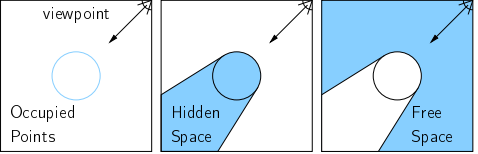
\includegraphics[width=0.9\linewidth]{\FIGDIR/10_Lidar_sets1.PNG} 
    \caption{Space type definitions}
    \label{fig:Spacetypes}
    \end{subfigure}
    \begin{subfigure}{0.5\textwidth}
    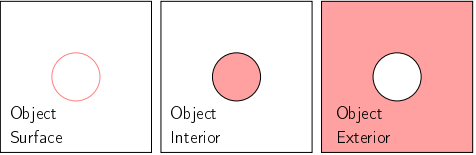
\includegraphics[width=0.9\linewidth]{\FIGDIR/11_Lidar_sets2.PNG}
    \caption{Object properties definitions}
    \label{fig:ObectProperties}
    \end{subfigure}
    \caption{Six spaces of interest \cite{yapo2008probabilistic}}
    \label{fig:Spaces of interests}
 \end{figure}
 
\noindent  Because of real-time obstacle avoidance it is necessary to introduce following terminology:
\begin{enumerate}
    \item \textit{Occupied points} - points which have been detected by LiDAR (also addressed as visible points).
    \item \textit{Hidden space} - space which is hidden behind occupied points, from viewpoint it is uncertain what is in that space. 
    \item \textit{Free space} - space which is visible from viewpoint and it is not occupied by known objects.
    \item \textit{Object surface} - detected and undetected object surface
    \item \textit{Object interior} - occupied space by object.
    \item \textit{Object exterior} - free space around known objects.
\end{enumerate}
Existing method for space segregation \cite{yapo2008probabilistic} can yeld to following definition.
\begin{definition}[Accessible space]\label{def:accessibleSpace}
    Consider known space $S$ as space explored by sensor (it can have different viewpoint along previous 3D trajectory).
    Intersection between \textit{object exterior} $S_E$ and \textit{free space}$S_F$ gives us \textit{Accessible space}.
    \begin{equation}
        S_A = S_E \cap S_F
    \end{equation}
\end{definition}
 
 \noindent Accessible space $S_A$ (\ref{def:accessibleSpace}) is our bordering limitation for reachable space of system $R(\tau,t_0,\vec{x_0})$ (def. \ref{def:reachset01}.); 

 
\section{Complements of algebra}

\noindent 3D Cartesian space gives us an x, y, and z axis (describing position based on horizontal placement, vertical placement, and depth respectively). The coordinates for any point within this space are shown as a tuple $(x,y,z)$. Coordinate system used this work will be viewed as right-handed system (thumbs points at positive direction of x-axis, index finger is pointing to positive direction of y-axis, then positive  direction of z axis is shown by remaining fingers).

Euler have worked on universal rotation theorem which was presented in \cite{euler1775formulae}. Rigid body dynamics and rotation matrices have been proposed in book by Schaub \cite{schaub2003analytical}. Local coordinates are used, where plane center of gravity is used as center point and plane heading is oriented to X axis. This local coordinate system is called Euler Normalized Unit-frame (ENU). Rotation matrices are used to transform between two displaced coordinate systems. Roll angle $\alpha$ rotation is defined around X-axis by matrix (\ref{eq:rollTransformationMatrix}) on YZ-plane. Pitch angle $\beta$ rotation matrix is defined around Y-axis by matrix (\ref{eq:pitchTransformationMatrix}) on XZ plane. Yaw angle $\gamma$ rotation matrix is defined around Z axis by matrix (\ref{eq:yawTranformationMatrix}) on XY plane.

\begin{equation}\label{eq:rollTransformationMatrix}
    R_{YZ} = R_\alpha =
    \begin{bmatrix}
        1 & 0 & 0\\
        0 & \cos(\alpha) & -\sin(\alpha)\\
        0 & \sin(\alpha) & \cos(\alpha)
    \end{bmatrix}
\end{equation}
\begin{equation}\label{eq:pitchTransformationMatrix}
    R_{XZ} = R_\beta =
    \begin{bmatrix}
        \cos(\beta) & 0 & \sin(\beta)\\
        0 & 1 & 0\\
        -\sin(\beta) & 0 & \cos(\beta)
    \end{bmatrix}
\end{equation}
\begin{equation}\label{eq:yawTranformationMatrix}
    R_{XY} = R_\gamma = 
    \begin{bmatrix}
        \cos(\gamma) & -\sin(\gamma) & 0 \\
        \sin(\gamma) & \cos(\gamma) & 1 \\
        0 & 0 & 1
    \end{bmatrix}
\end{equation}
Final rotation matrix in XYZ ordered space is given by equation(\ref{eq:xyzspaceRotationMatrix}).
\begin{equation}\label{eq:xyzspaceRotationMatrix}
    \begin{aligned}
        R_{XYZ}  =& R_{\alpha\beta\gamma} =  R_{XY} * R_{XZ} * R_{YZ} = R_\gamma * R_\beta *R_\alpha\\
         =& 
         \small
         \begin{bmatrix}
            \cos\beta\cos\gamma & \cos\gamma\sin\alpha\sin\beta - \cos\alpha\sin\gamma & \sin\alpha\sin\gamma + \cos\alpha\cos\gamma\sin\beta \\
            \cos\beta\sin\gamma & \cos\alpha\cos\gamma + \sin\alpha\sin\beta\sin\gamma & \cos\alpha\sin\beta\sin\gamma - \cos\gamma\sin\alpha \\
            -\sin\beta & \cos\beta\sin\alpha & \cos\alpha\cos\beta 
         \end{bmatrix}
         \normalsize
    \end{aligned}
\end{equation}
To keep solution numerically stable and rotations numerically stable gimbal lock prevention is necessary \cite{kramer1977gyro}. Gimbal lock occurs when one of matrices (\ref{eq:rollTransformationMatrix}, \ref{eq:pitchTransformationMatrix}, \ref{eq:yawTranformationMatrix}) is singular or final matrix for XYZ rotation is singular (\ref{eq:xyzspaceRotationMatrix}). Gimbal lock leads to loose of one or more degree of freedom, depending on rank and space dimension of singular matrix. To prevent gimbal lock it is necessary to introduce mechanism to check if rotation matrix is regular. For this purpose normative reset function is introduced:
\begin{equation}
    \left [ \alpha, \beta ,\gamma \right ]^T = f(t,\alpha^-,\beta^-,\gamma^-), \quad \textnormal{norm}(R_{\alpha\beta\gamma})=3
\end{equation}
Function resets yaw $\gamma$ or roll $\alpha$ angle to initial position to keep degree of rotation matrix. Simpler but not fault tolerant solution is to keep angles $\alpha,\beta,\gamma, \in \left (  -\pi,\pi\right ]$ range.

\subsection{Transformation between coordinate systems}
\noindent Polar coordinate system represents point in form of vector $[distance$, $angle_{horizontal}$, $angle_{vertical}]$, which is ideal for representation of LiDAR scanned point, because usually total point distance andpair of angles are returned. Using most common LiDAR with horizontal rotation $\theta$ and vertical mirror inclination $\varphi$, one can define planar coordinate $p_{planar} = [d_{xyz},\theta,\varphi]$ which is dual to Cartesian coordinate $p_{cartesian} = [x,y,z]$. If rotation angles are forced to stay as $\theta,\varphi\in(-\pi,\pi]$ transformation function is bijection.

Transformation from planar to Cartesian representation is defined by following series of functions (\ref{eq:cpt01}, \ref{eq:cpt02},\ref{eq:cpt03}, \ref{eq:cpt04}).
\begin{equation}\label{eq:cpt01}
    d_{xy} = \cos\varphi.d_{xyz}
\end{equation}
\begin{equation}\label{eq:cpt02}
    z = \sin\varphi.d_{xyz}
\end{equation}
\begin{equation}\label{eq:cpt03}
    y = \sin\theta.d_{xy}
\end{equation}
\begin{equation}\label{eq:cpt04}
    x = \cos\theta.d_{xy}
\end{equation}
Transformation from Cartesian to planar representation is defined by following series of functions (\ref{eq:cpt05}, \ref{eq:cpt06},\ref{eq:cpt07}, \ref{eq:cpt08}).
\begin{equation}\label{eq:cpt05}
    d_{xyz} = \sqrt{x^2+y^2+z^2}    
\end{equation}
\begin{equation}\label{eq:cpt06}
    d_{xy} = \sqrt{x^2+y^2}    
\end{equation}
\begin{equation}\label{eq:cpt07}
    \theta = \arctan\frac{y}{x}
\end{equation}
\begin{equation}\label{eq:cpt08}
    \varphi= \arctan\frac{z}{d_{xy}}
\end{equation}

\begin{definition}{Global coordinate system $\mathscr{X}_\mathscr{G}$}\label{def:globalCoordinateSystem}
    takes as center $c_{\mathscr{G}0}$ well known point (for example center of geo-reference model in GNSS systems) every reference distance, plane or angle is calculated taking this center to mind.
\end{definition}
\begin{definition}{Local coordinate system $\mathscr{X}_\mathscr{L}$}\label{def:localCoordinateSystem}
    takes as center $c_{\mathscr{L}0}$ frame of vehicle and can be changing position and orientation in global coordinate frame $\mathscr{X}_\mathscr{G}$.
\end{definition}
\begin{definition}{Global position of planar obstacle $o_i\in\mathscr{O}_{3D}$.}\label{def:globalObstaclePosition3D}
    Let $o_i = [d_o, \theta_o, \varphi_o]^T$ be planar position of obstacle $o_i$ in local coordinate frame of vehicle with global Cartesian position $[x,_v,y_v,z_v]^T$ and normalized orientation angles $[\alpha_v,\beta_v,\gamma_v]$.\\
    Then Cartesian position of obstacle $oi$, $[x_o,y_o,z_o]^T$  in local coordinate frame is given by transformation functions $x_o$ (\ref{eq:cpt04}), $y_o$ (\ref{eq:cpt03}), $z_o$ (\ref{eq:cpt02}).\\ 
    Global  position of planar obstacle $oi$, $[x_g,y_g,z_g]^T$ is given by following equation:
    \begin{equation}
        \begin{bmatrix}
            x_g\\y_g\\z_g
        \end{bmatrix}
        =
        \left [
            R_{XYZ}(\alpha_v,\beta_v,\gamma_v)
            \begin{bmatrix}
                x_o\\y_o\\z_o
            \end{bmatrix}
            +
            \begin{bmatrix}
                x_v\\y_v\\z_v
            \end{bmatrix}
        \right ]
    \end{equation}    
\end{definition}

\begin{definition}{Local position of global coordinate $[x_g,y_g,z_g]^T\in\R^3$.}\label{def:globalToLocal}
    Let there be vehicle with global Cartesian position $[x,_v,y_v,z_v]^T$ and normalized orientation angles $[\alpha_v,\beta_v,\gamma_v]$. in global coordinate frame $\mathscr{X}_\mathscr{X}$.\\
    Then local Cartesian coordinate position $[x_l,y_l,z_l]^T$ of point $[x_g,y_g,z_g]^T$ is given by following equation:
    \begin{equation}
        \begin{bmatrix}
            x_l\\y_l\\z_l
        \end{bmatrix}
        =
        \left [
            R_{XYZ}(-\alpha_v,-\beta_v,-\gamma_v)
            \left (
            \begin{bmatrix}
                x_g\\y_g\\z_g
            \end{bmatrix}
            -
            \begin{bmatrix}
                x_v\\y_v\\z_v
            \end{bmatrix}
            \right )
        \right ]
    \end{equation}
    Local planar position is given as $[d_l, \theta_l,\varphi_l]$, where $d_l$ is given by (\ref{eq:cpt05}), $\theta_l$ is givent by (\ref{eq:cpt07}). $\varphi_l$ is given by (\ref{eq:cpt08}), where $[x_l,y_l,z_l]$ are used as local coordinates.
\end{definition}

\subsection{Planar surface calculation}
\noindent The problem is to calculate intersected surface $dA$ of ball subsurface defined by radius $r$, horizontal span $\phi$ and vertical span $\theta$. From clasicall mechanics one can formulate problem as given by figure \ref{fig:80BallSpan}. The intersection plot is in figure \ref{fig:81BallSpan2}.
\begin{figure}[H]
    \centering
    \begin{subfigure}[H]{0.3\textwidth}
        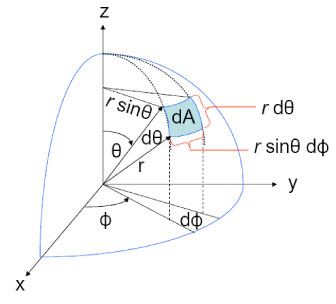
\includegraphics[width=\textwidth]{\FIGDIR/80BallSpan.jpg}
        \caption{Notation}
        \label{fig:80BallSpan}
    \end{subfigure}
    \begin{subfigure}[H]{0.3\textwidth}
        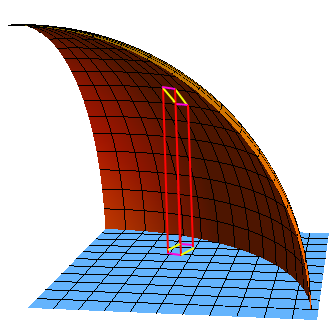
\includegraphics[width=\textwidth]{\FIGDIR/81BallSpan2.png}
        \caption{Plot}
        \label{fig:81BallSpan2}
    \end{subfigure}
    \caption{Planar surface calculation notation and plot}
    \label{fig:BallSpanNOTPLOT}
\end{figure}

\noindent One can use first fundamental form to determine the surface area element. Recall that this is the metric tensor, whose components are obtained by taking the inner product of two tangent vectors in planar space $g_{i,j}= X_i \cdot X_j$, for tangent vectors $X_i$, $X_j$. Following identification for the components of metric tensor will be used:
\begin{equation}\label{eq:metricTensorIdentification}
    g_{ij}=
    \begin{bmatrix}
        E&F\\
        F&G
    \end{bmatrix}
\end{equation}

\noindent Where $E=<X_u,X_u>$, $F=<X_u,X_v>$, and $G=<X_v,X_v>$. Lagrange`s identity can be used , which tells us that the squared area of a parallelogram in space is equal to the sum of the squares of its projections onto the Cartesian plane:
\begin{equation}\label{eq:CartesianProjectionIdentity}
    |X_u \times X_v|^2 = |X_u|^2|X_v|^2 - \left(X_u\cdot X_v\right)^2
\end{equation}

\noindent Given example is displayed in figure \ref{fig:81BallSpan2}. The area element is given as:
\begin{equation}\label{eq:squareElementSurfaceDerivation}
    \begin{aligned}
    \text{d}A &= |X_u \times X_v| \quad\text{d}u\text{d}v \\
    & = \sqrt{\left||X_u|^2|X_v|^2 - \left(X_u\cdot X_v\right)^2\right|}\quad \text{d}u\text{d}v\\ 
    & = \sqrt{EG-F^2} \quad \text{d}u\text{d}v
    \end{aligned}
\end{equation}

\noindent We will find tangent vectors via the usual parametrization which give, $X(\phi,\theta)$ = $[r \cos\phi\sin\theta,$ $r\sin\phi\sin\theta,$ $r\cos\theta]$, so that tangent vectors are simply defined as:
\begin{equation}\label{eq:tangentVectorsForPlanarSurface}
    \begin{aligned}
        X_\phi &= [-r\sin\phi\cos\theta,r\cos\phi\sin\theta,0]\\
        X_\theta &=[-r\cos\phi\sin\theta,r\sin\phi\cos\theta,-r\sin\theta]
    \end{aligned}
\end{equation}

\noindent Computing the elements of the first fundamental form gives us:
\begin{equation}
    E = r^2\cos^2\theta,\quad F=0,\quad G=r^2
\end{equation}

\noindent Thus final difference is given as:
\begin{equation}\label{eq:finalCellSquare}
    \text{d}A=\sqrt{r^4\cos^2}\quad \text{d}\theta\text{d}\phi = r^2 \cos\theta\quad \text{d}\theta\text{d}\phi
\end{equation}
